\documentclass[12pt]{article}
\usepackage[utf8]{inputenc}
\usepackage[margin=1in]{geometry}
\usepackage{amsmath}\usepackage{amssymb}\usepackage{multicol}\usepackage{enumitem}
\usepackage{pgfplots}\pgfplotsset{compat=1.17}
\setlength{\parindent}{0pt}
\begin{document}

\fbox{\parbox{0.97\linewidth}{\small\textbf{Final answers} (record here --- graded on the answer; show your work):\\[6pt]1.~\underline{\hspace{1.5cm}}\quad 2.~\underline{\hspace{1.5cm}}\quad 3.~\underline{\hspace{1.5cm}}\quad 4.~\underline{\hspace{1.5cm}}\quad 5.~\underline{\hspace{1.5cm}}\quad 6.~\underline{\hspace{1.5cm}}\quad 7.~\underline{\hspace{1.5cm}}\quad 8.~\underline{\hspace{1.5cm}}\quad 9.~\underline{\hspace{1.5cm}}}}
\vspace{0.35cm}

\begin{center}{\Large \textbf{Increasing, Decreasing, Max \& Min}}\end{center}\vspace{0.2cm}
% State max/min, vertex, and intervals
\textbf{Example (State max/min, vertex, and intervals):}

For $y=x^{2}-4$, vertex form gives vertex $(0,-4)$. Leading coefficient $+1$ is positive, so it's a \textbf{minimum}. It decreases for $x<0$ and increases for $x>0$.

\begin{center}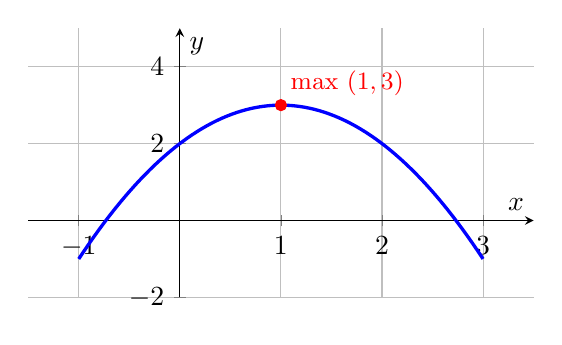
\begin{tikzpicture}
\begin{axis}[axis lines=middle,xlabel=$x$,ylabel=$y$,xmin=-1.5,xmax=3.5,ymin=-2,ymax=5,width=8cm,height=5cm,grid=both,samples=80]
\addplot[very thick,blue,domain=-1:3]{-(x-1)^2+3};
\addplot[only marks,mark=*,red] coordinates {(1,3)};
\node[above right,red,font=\small] at (axis cs:1,3) {max $(1,3)$};
\end{axis}\end{tikzpicture}\end{center}
{\small\centering $y=-(x-1)^2+3$ --- opens down, so the vertex is a maximum.\par}
\vspace{0.2cm}\hrule\vspace{0.35cm}
\textbf{Directions: State max or min, give the vertex, and give both intervals using inequality notation.}

\begin{multicols}{2}
\begin{enumerate}[label=\textbf{\arabic*.}, start=1, itemsep=3cm]
  \item $\displaystyle y=x^{2}+5$
  \item $\displaystyle y=-x^{2}+1$
  \item $\displaystyle y=(x-3)^{2}$
  \item $\displaystyle y=-(x+2)^{2}-1$
  \item $\displaystyle y=(x+4)^{2}-6$
  \item $\displaystyle y=-(x-1)^{2}+3$
  \item $\displaystyle y=x^{2}-8x$
  \item \textbf{(challenge)}\ $\displaystyle y=2(x-3)^{2}+1$
\end{enumerate}
\end{multicols}

\vspace{0.2cm}\hrule\vspace{0.3cm}
\textbf{Challenge} (same sheet):\\[4pt]
\begin{enumerate}[label=\textbf{\arabic*.}, start=9, itemsep=2.2cm]
  \item \textbf{(challenge)}\ For $y=-2(x+3)^{2}+7$, find the vertex, state max or min, give both intervals, AND explain what would change about your answer if the leading coefficient became positive instead.
\end{enumerate}

\newpage

\begin{center}{\Large \textbf{Answer Key --- fully worked}}\end{center}
\vspace{0.25cm}
\textbf{Procedure:} Write the equation in vertex form $a(x-h)^2+k$ if it isn't already.; The vertex is $(h,k)$.; If $a>0$ the parabola opens up (minimum); if $a<0$ it opens down (maximum).; The graph decreases before the vertex and increases after it (for a minimum) --- reversed for a maximum..\\[8pt]
\begin{enumerate}[label=\textbf{\arabic*.},itemsep=7pt]
  \item Opens up, minimum; vertex $(0,5)$; decreasing $x<0$, increasing $x>0$
  \item Opens down, maximum; vertex $(0,1)$; increasing $x<0$, decreasing $x>0$
  \item Opens up, minimum; vertex $(3,0)$; decreasing $x<3$, increasing $x>3$
  \item Opens down, maximum; vertex $(-2,-1)$; increasing $x<-2$, decreasing $x>-2$
  \item Opens up, minimum; vertex $(-4,-6)$; decreasing $x<-4$, increasing $x>-4$
  \item Opens down, maximum; vertex $(1,3)$; increasing $x<1$, decreasing $x>1$
  \item Complete the square: $x^2-8x=(x-4)^2-16$; minimum; vertex $(4,-16)$; decreasing $x<4$, increasing $x>4$
  \item $a=2>0$ opens up, minimum; vertex $(3,1)$; decreasing $x<3$, increasing $x>3$
  \item Vertex form $a(x-h)^2+k$ gives vertex $(-3,7)$. Since $a=-2<0$ the parabola opens down, so $(-3,7)$ is a maximum. It increases on $x<-3$ and decreases on $x>-3$. If the leading coefficient became positive (e.g. $+2$), the parabola would open up instead: the vertex $(-3,7)$ would become a minimum, and the intervals would flip --- decreasing on $x<-3$ and increasing on $x>-3$.
\end{enumerate}

\end{document}